% Options for packages loaded elsewhere
\PassOptionsToPackage{unicode}{hyperref}
\PassOptionsToPackage{hyphens}{url}
%
\documentclass[
  american,
]{article}
\usepackage{lmodern}
\usepackage{amssymb,amsmath}
\usepackage{ifxetex,ifluatex}
\ifnum 0\ifxetex 1\fi\ifluatex 1\fi=0 % if pdftex
  \usepackage[T1]{fontenc}
  \usepackage[utf8]{inputenc}
  \usepackage{textcomp} % provide euro and other symbols
\else % if luatex or xetex
  \usepackage{unicode-math}
  \defaultfontfeatures{Scale=MatchLowercase}
  \defaultfontfeatures[\rmfamily]{Ligatures=TeX,Scale=1}
\fi
% Use upquote if available, for straight quotes in verbatim environments
\IfFileExists{upquote.sty}{\usepackage{upquote}}{}
\IfFileExists{microtype.sty}{% use microtype if available
  \usepackage[]{microtype}
  \UseMicrotypeSet[protrusion]{basicmath} % disable protrusion for tt fonts
}{}
\makeatletter
\@ifundefined{KOMAClassName}{% if non-KOMA class
  \IfFileExists{parskip.sty}{%
    \usepackage{parskip}
  }{% else
    \setlength{\parindent}{0pt}
    \setlength{\parskip}{6pt plus 2pt minus 1pt}}
}{% if KOMA class
  \KOMAoptions{parskip=half}}
\makeatother
\usepackage{xcolor}
\IfFileExists{xurl.sty}{\usepackage{xurl}}{} % add URL line breaks if available
\IfFileExists{bookmark.sty}{\usepackage{bookmark}}{\usepackage{hyperref}}
\hypersetup{
  pdftitle={Automatic Music Transcription},
  pdfauthor={Rand ASSWAD},
  pdflang={en-US},
  hidelinks,
  pdfcreator={LaTeX via pandoc}}
\urlstyle{same} % disable monospaced font for URLs
\usepackage[margin=1in]{geometry}
\usepackage{color}
\usepackage{fancyvrb}
\newcommand{\VerbBar}{|}
\newcommand{\VERB}{\Verb[commandchars=\\\{\}]}
\DefineVerbatimEnvironment{Highlighting}{Verbatim}{commandchars=\\\{\}}
% Add ',fontsize=\small' for more characters per line
\usepackage{framed}
\definecolor{shadecolor}{RGB}{248,248,248}
\newenvironment{Shaded}{\begin{snugshade}}{\end{snugshade}}
\newcommand{\AlertTok}[1]{\textcolor[rgb]{0.94,0.16,0.16}{#1}}
\newcommand{\AnnotationTok}[1]{\textcolor[rgb]{0.56,0.35,0.01}{\textbf{\textit{#1}}}}
\newcommand{\AttributeTok}[1]{\textcolor[rgb]{0.77,0.63,0.00}{#1}}
\newcommand{\BaseNTok}[1]{\textcolor[rgb]{0.00,0.00,0.81}{#1}}
\newcommand{\BuiltInTok}[1]{#1}
\newcommand{\CharTok}[1]{\textcolor[rgb]{0.31,0.60,0.02}{#1}}
\newcommand{\CommentTok}[1]{\textcolor[rgb]{0.56,0.35,0.01}{\textit{#1}}}
\newcommand{\CommentVarTok}[1]{\textcolor[rgb]{0.56,0.35,0.01}{\textbf{\textit{#1}}}}
\newcommand{\ConstantTok}[1]{\textcolor[rgb]{0.00,0.00,0.00}{#1}}
\newcommand{\ControlFlowTok}[1]{\textcolor[rgb]{0.13,0.29,0.53}{\textbf{#1}}}
\newcommand{\DataTypeTok}[1]{\textcolor[rgb]{0.13,0.29,0.53}{#1}}
\newcommand{\DecValTok}[1]{\textcolor[rgb]{0.00,0.00,0.81}{#1}}
\newcommand{\DocumentationTok}[1]{\textcolor[rgb]{0.56,0.35,0.01}{\textbf{\textit{#1}}}}
\newcommand{\ErrorTok}[1]{\textcolor[rgb]{0.64,0.00,0.00}{\textbf{#1}}}
\newcommand{\ExtensionTok}[1]{#1}
\newcommand{\FloatTok}[1]{\textcolor[rgb]{0.00,0.00,0.81}{#1}}
\newcommand{\FunctionTok}[1]{\textcolor[rgb]{0.00,0.00,0.00}{#1}}
\newcommand{\ImportTok}[1]{#1}
\newcommand{\InformationTok}[1]{\textcolor[rgb]{0.56,0.35,0.01}{\textbf{\textit{#1}}}}
\newcommand{\KeywordTok}[1]{\textcolor[rgb]{0.13,0.29,0.53}{\textbf{#1}}}
\newcommand{\NormalTok}[1]{#1}
\newcommand{\OperatorTok}[1]{\textcolor[rgb]{0.81,0.36,0.00}{\textbf{#1}}}
\newcommand{\OtherTok}[1]{\textcolor[rgb]{0.56,0.35,0.01}{#1}}
\newcommand{\PreprocessorTok}[1]{\textcolor[rgb]{0.56,0.35,0.01}{\textit{#1}}}
\newcommand{\RegionMarkerTok}[1]{#1}
\newcommand{\SpecialCharTok}[1]{\textcolor[rgb]{0.00,0.00,0.00}{#1}}
\newcommand{\SpecialStringTok}[1]{\textcolor[rgb]{0.31,0.60,0.02}{#1}}
\newcommand{\StringTok}[1]{\textcolor[rgb]{0.31,0.60,0.02}{#1}}
\newcommand{\VariableTok}[1]{\textcolor[rgb]{0.00,0.00,0.00}{#1}}
\newcommand{\VerbatimStringTok}[1]{\textcolor[rgb]{0.31,0.60,0.02}{#1}}
\newcommand{\WarningTok}[1]{\textcolor[rgb]{0.56,0.35,0.01}{\textbf{\textit{#1}}}}
\usepackage{longtable,booktabs}
% Correct order of tables after \paragraph or \subparagraph
\usepackage{etoolbox}
\makeatletter
\patchcmd\longtable{\par}{\if@noskipsec\mbox{}\fi\par}{}{}
\makeatother
% Allow footnotes in longtable head/foot
\IfFileExists{footnotehyper.sty}{\usepackage{footnotehyper}}{\usepackage{footnote}}
\makesavenoteenv{longtable}
\usepackage{graphicx}
\makeatletter
\def\maxwidth{\ifdim\Gin@nat@width>\linewidth\linewidth\else\Gin@nat@width\fi}
\def\maxheight{\ifdim\Gin@nat@height>\textheight\textheight\else\Gin@nat@height\fi}
\makeatother
% Scale images if necessary, so that they will not overflow the page
% margins by default, and it is still possible to overwrite the defaults
% using explicit options in \includegraphics[width, height, ...]{}
\setkeys{Gin}{width=\maxwidth,height=\maxheight,keepaspectratio}
% Set default figure placement to htbp
\makeatletter
\def\fps@figure{htbp}
\makeatother
\setlength{\emergencystretch}{3em} % prevent overfull lines
\providecommand{\tightlist}{%
  \setlength{\itemsep}{0pt}\setlength{\parskip}{0pt}}
\setcounter{secnumdepth}{5}
\geometry{paper=a4paper, margin=2.2cm}
\usepackage[defaultlines=10,all]{nowidow}
\usepackage{float}
\usepackage[justification=centering]{caption}

% force babel to use default item labels
%\frenchbsetup{StandardItemLabels=true}

% tables
\usepackage{boldline} % provides V{n} and \hlineB{n}
\usepackage{makecell} % for line breaks inside cell
\usepackage{multirow} % for multirow cells

% math
%\usepackage{amsmath}
%\usepackage{amsthm,amssymb,amsfonts,amscd}
%\usepackage{mathtools}
%\usepackage{centernot}

% music characters
\usepackage{musicography}
\DeclareUnicodeCharacter{266F}{\musSharp{}}
\DeclareUnicodeCharacter{266D}{\musFlat{}}
\DeclareUnicodeCharacter{266E}{\musNatural{}}

% remove paragraph numbering
\let\oldparagraph\paragraph
\renewcommand{\paragraph}[1]{\oldparagraph*{#1}}

\makeatletter

\usepackage{fancyhdr}
\pagestyle{fancy}
\lhead{Automatic Music Transcription}
\rhead{Rand ASSWAD}

\usepackage{pmboxdraw} % for tree chars encoding

\renewcommand{\fps@figure}{H}

\AtBeginDocument{\let\maketitle\relax}

%%%%%%%%%%%%%%%% COVER

\setlength{\parindent}{0cm}
\setlength{\parskip}{1ex plus 0.5ex minus 0.2ex}
\newcommand{\hsp}{\hspace{20pt}}
\newcommand{\HRule}{\rule{\linewidth}{0.5mm}}
\ifxetex
  % Load polyglossia as late as possible: uses bidi with RTL langages (e.g. Hebrew, Arabic)
  \usepackage{polyglossia}
  \setmainlanguage[variant=american]{english}
\else
  \usepackage[shorthands=off,main=american]{babel}
\fi
\newlength{\cslhangindent}
\setlength{\cslhangindent}{1.5em}
\newenvironment{cslreferences}%
  {\setlength{\parindent}{0pt}%
  \everypar{\setlength{\hangindent}{\cslhangindent}}\ignorespaces}%
  {\par}

\title{Automatic Music Transcription}
\usepackage{etoolbox}
\makeatletter
\providecommand{\subtitle}[1]{% add subtitle to \maketitle
  \apptocmd{\@title}{\par {\large #1 \par}}{}{}
}
\makeatother
\subtitle{Masters Thesis Project}
\author{Rand ASSWAD}
\date{12 March 2020}

\begin{document}
\maketitle

\begin{titlepage}
    \begin{sffamily}
        \begin{center}
            \begin{minipage}[c]{0.45\textwidth}
            \raggedright
\includegraphics[height=2cm]{img/logo_insa.png}
            \end{minipage}~\hfill~%
            \begin{minipage}[c]{0.45\textwidth}
            \raggedleft
\includegraphics[height=1.75cm]{img/logo_univ.png}
            \end{minipage}\\[2cm]

            \textsc{\huge Masters Thesis Project}\\[1cm]

            % Title
            \HRule \\[0.4cm]
            {\huge \bfseries Automatic Music Transcription \\[0.4cm]}
            \HRule \\[1cm]
            
            \textsc{\huge Audio Signal Processing}\\[1cm]

            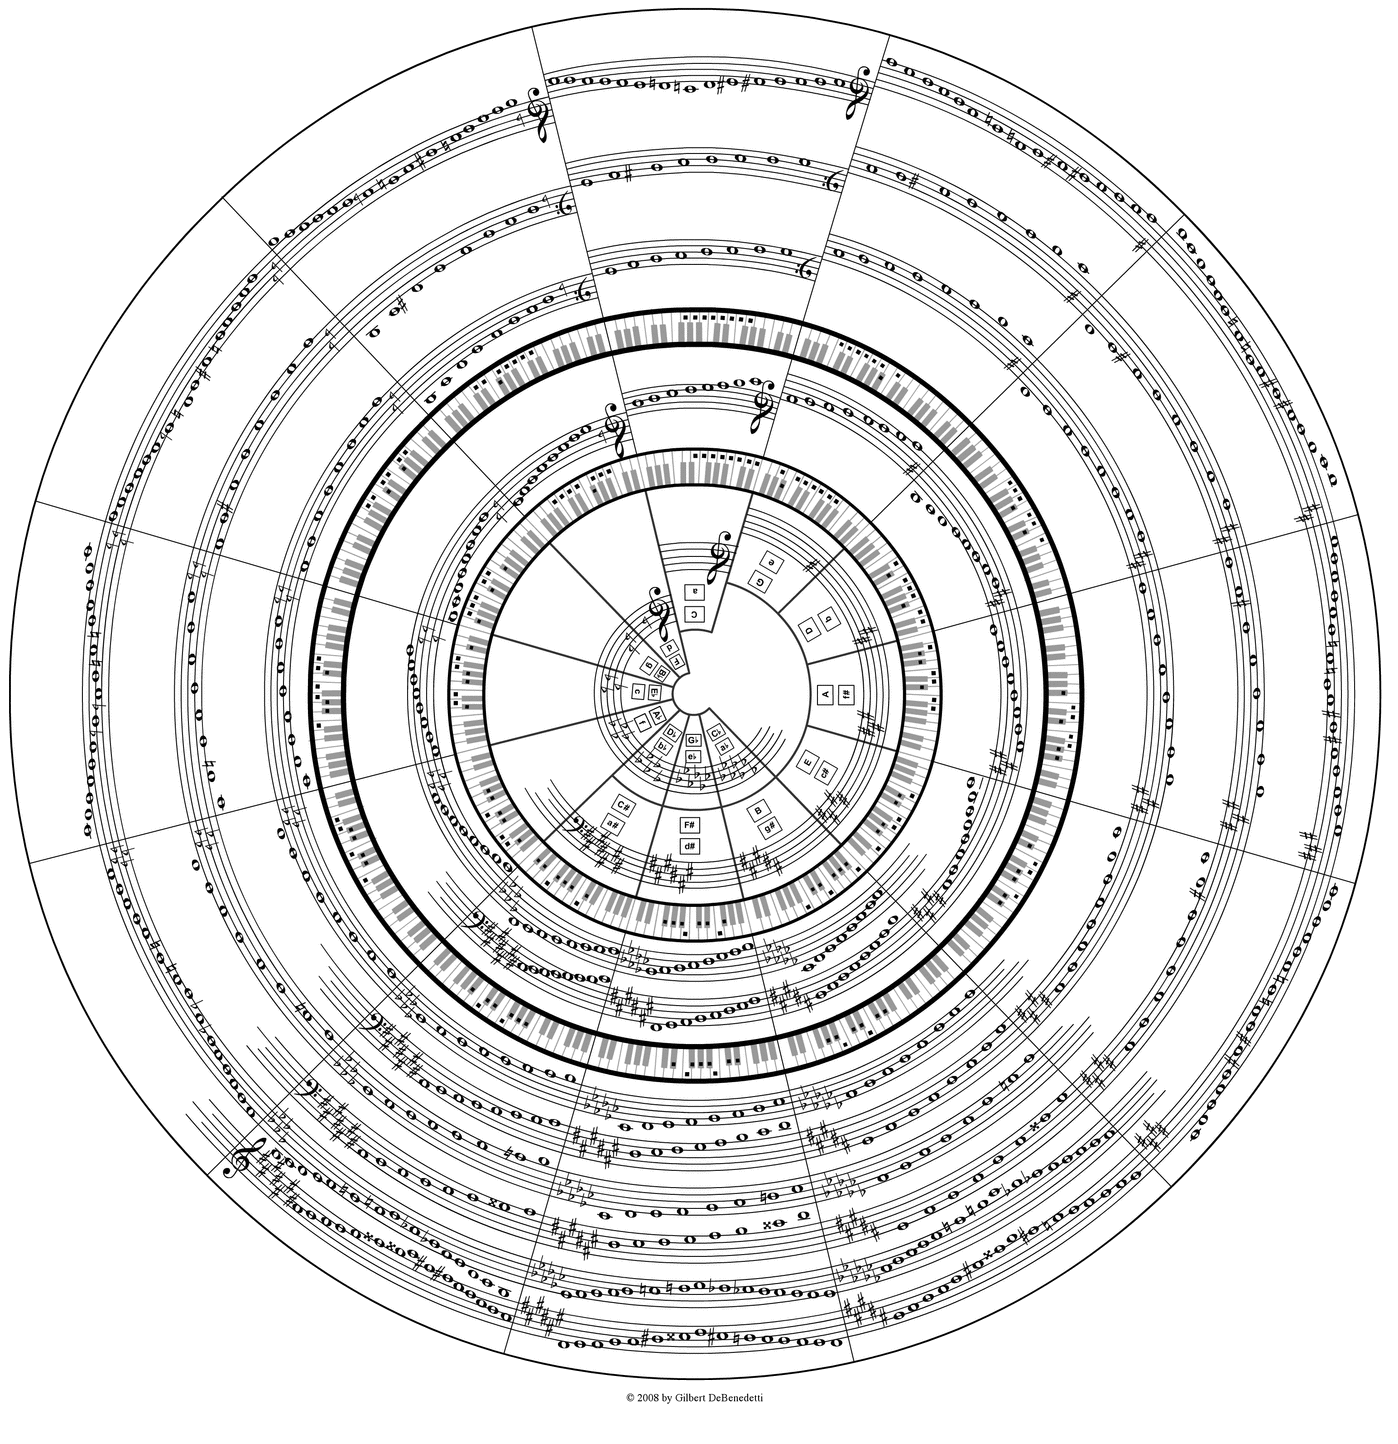
\includegraphics[width=.6\textwidth]{img/cover_img.png}~\\[2cm]

            % Author and supervisor
            \begin{minipage}{0.45\textwidth}
            \begin{flushleft} \large
                Rand ASSWAD\\
                Department of Applied Mathematics\\
                Theoretical and Applied Computer Science
            \end{flushleft}
            \end{minipage}
            \begin{minipage}{0.45\textwidth}
            \begin{flushright} \large
                \emph{Under the supervision of:}\\
                Prof. Natalie FORTIER\\
                Prof. Jean-Philippe DUBERNARD
            \end{flushright}
            \end{minipage}

            \vfill
            % Bottom of the page
            {\large 12 March 2020}
        \end{center}
    \end{sffamily}
\end{titlepage}
\makeatother

{
\setcounter{tocdepth}{3}
\tableofcontents
}
\def\R{\mathbb{R}}
\def\C{\mathbb{C}}
\def\N{\mathbb{N}}
\def\Z{\mathbb{Z}}

\def\x{\tilde{x}}
\def\w{\omega}
\def\phi{\varphi}

\def\dt{\mathrm{d}t}

\def\pp#1{\left(#1\right)}
\def\sset#1{\left\{#1\right\}}
\def\vset#1#2{\sset{#1\left\lvert#2\right.}}

\def\abs #1{\left\lvert#1\right\rvert}
\def\norm#1{\left\lVert#1\right\rVert}
\def\dotp#1#2{\left\langle#1{;}#2\right\rangle}

\def\pmat#1{\begin{pmatrix}#1\end{pmatrix}}

\def\qtext#1{\quad\text{#1}\quad}

\def\argmin{\mathop{\mathrm{argmin}}}
\def\argmax{\mathop{\mathrm{argmax}}}
\def\supp{\mathop{\mathrm{supp}}}

\def\transp#1{{#1}^{\top}}

\def\f{\boldsymbol{f}}
\def\ff{\f\hspace{-2pt}\f}
\def\mf{\boldsymbol{mf}}
\def\mp{\boldsymbol{mp}}
\def\p{\boldsymbol{p}}
\def\piu{pi\grave{u}~}

\def\X{\boldsymbol{X}}
\def\V{\boldsymbol{V}}
\def\W{\boldsymbol{W}}
\def\H{\boldsymbol{H}}

\pagebreak

\hypertarget{introduction}{%
\section*{Introduction}\label{introduction}}
\addcontentsline{toc}{section}{Introduction}

Music is ubiquitous ever since humans exist.
Prehistoric instruments have been found and thought to be at least
40,000 years old.
Music is a pilar of human civilisation; it relates to people's identities,
feelings and thoughts.
Hence, means of saving and sharing music are of invaluable importance.
The oldest surviving notated music work \emph{Hurrian Hymn to Nikkal}
found on clay tablets dates back to 1400 BC.

Various systems were developped around the globe for \emph{visually}
representing perceived music through the use of written symbols.
The modern western notation is the predominent musical notation
worldwide for most music genres.

With the rise of technology, audio recordings where introduced
as analog signals and eventually as digital signals,
providing means for sharing and sauveguarding music \emph{aurally}.

Music theory and musical notation have been studied for centuries,
allowing humans and machines to retrieve music information
from common formats.
Nevertheless, \emph{music processing} is a relatively young discipline
compared to other subdomains of signal processing such as speech
processing; while great results are achieved today in speech recognition,
the task of retreiving music information from audio recordings
is still far along.

\textbf{Automatic Music Transcription} (AMT) is the task of analyzing
musical audio signals and producing the corresponding musical scores.
This task has captured researchers interest in the late 20\textsuperscript{th} century
and has become a wide research discipline as many of the problems
in this domain remain unsolved.
furthermore, strides in the domain of AMT would apply to numerous
applications that can facilitate creating, sharing, and learning music.

The scope of this thesis is the domain of Automatic Music Transcription
and the underlying tasks.
We explore the state of the art and propose an implementation
for a subset of the presented methods.

\pagebreak

\hypertarget{background}{%
\section{Background}\label{background}}

The focus of this project is music information retrieval
from music audio signals.
In this section we go through the main problems in
the discipline of Automatic Music Transcription,
we study characteristics of musical elements,
human perception of music, and basic notions
of modern music theory.
We also review the main characteristics of a sound wave
as well as analytic tools for processing digital audio signals.
Furthermore, we establish the bridge between music
theory and physical properties of audio signals.

\hypertarget{automatic-music-transcription}{%
\subsection{Automatic Music Transcription}\label{automatic-music-transcription}}

\begin{quote}
AMT is the process of converting an acoustic musical
signal into some form of musical notation. (Benetos et al. \protect\hyperlink{ref-benetos_2013}{2013})
\end{quote}

\hypertarget{history-and-community}{%
\subsubsection{History and community}\label{history-and-community}}

The interest in the task of AMT has started in the late
20\textsuperscript{th} century, with researchers borrowing and adapting
concepts from the well-established domain of
\emph{speech-processing}.
Major strides have been made in the 21\textsuperscript{st} century,
particularly since the creation of the International
Society for Music Information Retrieval \textbf{(ISMIR)} in 2000.
Which have connected the community and provided a platform
for sharing and learning Music Information Retrieval \textbf{(MIR)}
concepts worldwide. (Müller \protect\hyperlink{ref-muller_2015}{2015})

furthermore, the Music Information Retrieval Evaluation eXchange
\textbf{(MIREX)} is an annual evaluation compaign for MIR algorithms.
Since it started in 2005, MIREX has served as a benchmark
for evaluating novelty algorithms and helped advance
MIR Research.

\hypertarget{motivation}{%
\subsubsection{Motivation}\label{motivation}}

MIR and AMT can be of great interest for different demographics.
First, most musicians stand to benefit from reliable
transcription algorithms as it can facilitate their tasks in
difficult cases or for the least accelerate the process.

Moreover, in many music genres such as Jazz, musical
notation is rarely used, therefore the exchange formats
are almost exclusively recordings of performances.
AMT would play a role in democratizing no-score music
for new learners and provide an easier canonical
format for exchanging music.

Another use of MIR is score-following software development
that include a cursor that follows real-time playing
indicating the correct and incorrect notes played
helping pupils practice and progress on their
own more efficiently, making the task of music learning
less painful.

Furthermore, MIR allows performing musicological analysis
directly on recordings, gaining access to much larger
databases compared to anotated music, which can also
be applied for various tasks such as music recognition
or melody recognition.

\hypertarget{underlying-tasks}{%
\subsubsection{Underlying tasks}\label{underlying-tasks}}

Automatic Music Transcription is divided into several subtasks
where each represents a research topic that fall
within the scope of Musical Information Retrieval.

The largest topic of MIR is tonal analysis, which
is based on analysing spectral features of audio signals,
and subsequently estimating \emph{pitch}, melody and harmony.
Despite the large interest in this topic and various
techniques applied, this task remains the core problem in AMT,
Exploration of main pitch analysis techniques is the
first part of this project.

Another main AMT task is \emph{temporal segmentation},
which relates consequently to rythme extraction and tempo
detection in melodic sounds. (Benetos et al. \protect\hyperlink{ref-benetos_2013}{2013})
This task pertains pertains to spectral features
as well as signal energy.
We expore this topic in the second part of this project.

Several more tasks are needed to fully transcribe a musical
piece, including: loudness estimation, instrument recognition,
rhythm detection, scale detection and harmony analysis.
In the scope of this project, we limit our study to
\emph{pitch analysis} and \emph{temporal segmentation}.

\hypertarget{physical-definition-of-acoustic-waves}{%
\subsection{Physical definition of acoustic waves}\label{physical-definition-of-acoustic-waves}}

Sound is generated by vibrating objects, these vibrations
cause oscillations of molecules in the medium.
The varying pressure propagates through the medium as a wave,
the pressure is therefore the solution of the wave
equation in time and space, also known as the acoustic
wave equation. (Feynman \protect\hyperlink{ref-feynman}{1965})
\[\Delta p =\frac{1}{c^2}\frac{\partial^2 p}{ {\partial t}^2}\]
where \(p\) is the accoustic pressure function of time and space
and \(c\) is the speed of sound propagation.
The wave equation can be solved analytically with the
separation of variables method, resulting in a \emph{sinusoidal
harmonic} solutions.

In audio signal processing, we are interested in the pressure
at the receptor's position (listener or microphone),
hence the pressure as a function of time.
An audio signal is therefore defined as the deviation
of pressure from the average pressure of the medium
at the receptor's position.

The pressure function being harmonic, the sound signal
is of the form
\[\tilde{x}(t) = \sum_{h=0}^{\infty} A_h \cos(2\pi hf_0t + \varphi_h)\]
where

\begin{itemize}
\tightlist
\item
  \(f_0\) is called the \textbf{fundamental frequency} of the signal,
\item
  \(h\) is the harmonic number,
\item
  \(A_h\) is the amplitude of the \(h^\text{th}\) harmonic,
\item
  \(\varphi_h\) is the phase of the \(h^\text{th}\) harmonic.
\end{itemize}

In many works this formula appears in terms of the angular
frequency \(\omega=2\pi f\), we denote as well
\(f_h = h f_0\) for \(h\geq 1\).

As harmonics represent proper multiples of the fundamental
frequency, \(h=0\) is excluded from the sum
\[\tilde{x}(t) = a_0 + \sum_{h=1}^{\infty} A_h \cos(2\pi hf_0t + \varphi_h)\]
with \(a_0 = A_0\cos(\varphi_0)\).

\hypertarget{perception-of-sound-and-music}{%
\subsection{Perception of sound and music}\label{perception-of-sound-and-music}}

The human auditory system is capable of distinguishing
intensities and frequencies of sound waves as well as
temporal features.
The inner ear is extremely sensitive to sound wave features,
the brain allows further analysis of these features.

Music theory defines and studies \emph{perceived features}
of music signals.
These features are based on the signal's intensity,
frequency, and time patterns.

In music theory, a \textbf{note} is a musical symbol that
represents the smallest musical object.
The note's attributes define the \emph{pitch} of the sound, its
\emph{relative duration} and its \emph{relative intensity}.

\hypertarget{fundamental-frequency-and-pitch}{%
\subsubsection{Fundamental frequency and pitch}\label{fundamental-frequency-and-pitch}}

Sound signals are periodic, therefore by definition there
exists a \(T>0\) such as
\[\forall t, \tilde{x}(t)=\tilde{x}(t+T)\]
which follows that there exists an infinite set of values of \(T>0\) that verify this property, indeed
\(\forall n\in\mathbb{N}, T'=nT, \tilde{x}(t)=\tilde{x}(t+T')\).
We define the period of a signal as the smallest positive
value of \(T\) for which the property holds.
The \textbf{fundamental frequency} \(f_0\) is defined formally
as the reciprocal of the period.
This definition holds for \emph{any} periodic signal,
regardless of its form.

In the case of sound wave, the \emph{perception of the fundamental
frequency} is referred to as the \textbf{pitch}.
Pitch is the defined as the \emph{tonal height} of a sound,
it is closely related to the fundamental frequency
however remaining a \emph{relative musical concept}
unlike the \(f_0\) of a signal that is an absolute
mathematical value.
In fact, the relation between pitch and \(f_0\)
is neither bijective nor invariant.

In music theory, pitch is defined on a discrete space
unlike the continuous frequency space.
Moreover, human perception of frequency is logarithmic
hence obtaining the \emph{next pitch} corresponds to the
multiplication of the frequency by a certain value \(r\).

Finally, the frequency of the reference pitch A\textsubscript{4}
is widely accepted today as \(440 Hz\) while in the baroque
era it was around \(415 Hz\) and \(440 Hz\) was the frequency
corresponding to A♯ pitch.
Even in modern day, variations of the pitch frequency
exist in different regions and even different orchestras!

\hypertarget{perception-of-intensity}{%
\subsubsection{Perception of intensity}\label{perception-of-intensity}}

Sound intensity is defined physically as the power carried
by sound waves per unit area, whereas sound pressure is
the local pressure deviation from the ambient atmospheric
pressure caused by a sound wave.
Human perception of intensity is directly sensitive to
sound pressure, it is measured in terms of \emph{sound pressure level} (SPL)
which is a logarithmic measure of sound pressure \(P\)
relative to the atmospheric pressure \(P_0\) measured
in decibels \(\mathrm{dB}\).
\[\mathrm{SPL} = 20\log_{10}\left(\frac{P}{P_0}\right) \mathrm{dB}\]

Nevertheless, sensitivity to sound intensity is variable
across different frequencies.
The subjective perception of sound pressure
is defined by a sound's \textbf{loudness} which is a function of
both SPL and frequency ranging from quiet to loud.

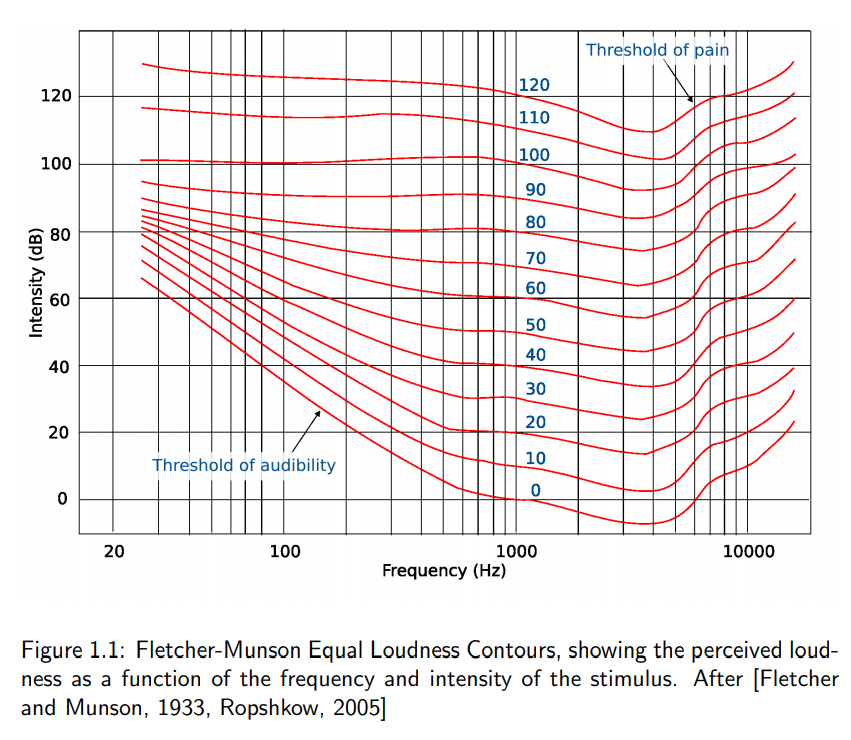
\includegraphics[width=0.6\textwidth,height=\textheight]{img/loudness.png}

In music theory, loudness is defined by a piece's \textbf{dynamics}.
Dynamics are indicators of a part's loudness \emph{relative}
to other parts and/or instruments.
Dynamics markings are expressed with the italian
keywords \emph{forte} \(\boldsymbol{f}\) (loud) and \emph{piano} \(\boldsymbol{p}\) (soft).
Subtle degrees of loudness can be expressed
by the prefixes \emph{mezzo-} or \emph{più}, for example \(\boldsymbol{mp}\) stands
for \emph{mezzo-piano} (moderately soft) and \(pi\grave{u}~\boldsymbol{p}\) (softer),
or by consecutive letters such as \emph{fortissimo} \(\boldsymbol{f}\hspace{-2pt}\boldsymbol{f}\)
(very loud) or more letters if needed.

Music dynamics also allow expressing gradual changes
in loudness, indicated as symbols or italian keywords
(\emph{crescendo} and \emph{diminuendo}).

\hypertarget{audio-signal-processing}{%
\subsection{Audio signal processing}\label{audio-signal-processing}}

\hypertarget{discrete-time-signals}{%
\subsubsection{Discrete-time signals}\label{discrete-time-signals}}

The domain of audio signal processing deals with recorded
digital/analog signals, which are discrete-time signals.
The \textbf{Nyquist-Shannon sampling theorem} is the fundamental
bridge between continuous-time and discrete-time signals.
It establishes a sufficient condition for a sample rate
that permits a discrete sequence of samples to capture
all the information from a continuous-time signal.
(Wikipedia \protect\hyperlink{ref-wiki:nyquistshannon}{2020})

The sample rate \(f_s\) of a discrete-time signal
is defined as the number of samples per second,
its inverse is the time step between samples \(T_s\).

We denote, conformely to litterature a discrete signal
time frame as \(x[n]=x(t_n)\) where
\(t_n=n\cdot T_s=\frac{n}{f_s}\).

\hypertarget{discrete-fourier-transform-dft}{%
\subsubsection{Discrete Fourier Transform (DFT)}\label{discrete-fourier-transform-dft}}

The discrete Fourier transform of \(N\) samples,
with a sample rate of \(f_s\) can be obtained
from its continuous definition.

\begin{align}
X(f) &= \int\limits_{0}^{t_N} x(t)\cdot e^{-2\pi j ft}\mathrm{d}t\\
    &= \lim\limits_{f_s\rightarrow\infty} \sum\limits_{n=0}^{N-1}
        x(t_n)\cdot e^{-2\pi j ft_n}\\
    &= \lim\limits_{f_s\rightarrow\infty} \underbrace{\sum\limits_{n=0}^{N-1} x[n]\cdot e^{-2\pi j f \frac{n}{f_s}}}_{X[f]}\\
    &= \lim\limits_{f_s\rightarrow\infty} X[f]
\end{align}

The DFT of \(x[n]\) is given for all frequency bins
\(k=0,\ldots,K\)
\[X[k] = \sum\limits_{n=0}^{N-1} x[n]\cdot e^{-2\pi j k \frac{n}{f_s}}\]

\pagebreak

\hypertarget{pitch-analysis}{%
\section{Pitch analysis}\label{pitch-analysis}}

\hypertarget{introduction-1}{%
\subsection{Introduction}\label{introduction-1}}

Pitch analysis is the task of estimating the fundamental
frequency of a periodic signal that is the inverse
of the period which is defined as
``the smallest positive member of the infinite set of time
shifts leaving the signal invariant'' (Cheveigné and Kawahara \protect\hyperlink{ref-yin_2002}{2002}).
As music signal frequencies vary through time,
the pitch analysis is usually performed on a short time frame (window)
allowing to express the obtained pitch as a function of time,
we will consider henceforth the analysis on a single frame.

Furthermore, the physical model we have considered
for the signal formula is based on physical hypotheses.
In fact, we considered a signal formed by a perfectly
harmonic instrument travelling in a perfectly undisturbed
homogenuous medium with no other iterfering waves.
Since such conditions are almost never met, we base our
analysis on \emph{imperfect conditions}.
Indeed, the recorded signal represents the pressure function
at the receptors position.
Consequently, the recorder captures the pressure
at its position from \emph{all} surrounding stimuli,
recording surrounding noise, resonance effects,
and the reflected wave with a certain lag.
As a result, we express the observed signal
as the sum of the harmonic signal \(\tilde{x}\) and
the residual \(z\). (Yeh \protect\hyperlink{ref-yeh_thesis}{2008})
\[x(t) = \tilde{x}(t) + z(t)\]

Before we move on, let's consider the \emph{harmonicity} of a sound.
In the case of perfectly harmonic instrument the frequency
of harmonic partials is expressed as a proper multiple
of the fundamental frequency \(f_h = h f_0\).
However, most musical instruments are not perfectly harmonic,
for example the \(h^\text{th}\) harmonic frequency
of a vibrating string is given as
\[ f_h = h f_0 \sqrt{1 + Bh^2} \quad\text{where}\quad
    B = \frac{\pi^3 Ed^4}{64l^2T}\]
where \(B\) is the inharmonicity factor of the string,
\(E\) is Young's modulus, \(d\) is the diameter of the string,
\(l\) is its length and \(T\) is its tension.
We refer to such signals as \textbf{quasi-periodic}.
Pitch analysis therefore has to take into account
the inharmonicity of a signal in the process of estimating
its fundamental frequencies in order to prevent
cases of false negatives (missed pitches).
{[}source needed{]}

Pitch analysis deals with both monophonic and polyphonic signals,
a monophonic signal is a signal produced by a single harmonic
source whereas polyphonic signals have multiple sources,
in the case of the latter the
task is significantly harder.
Nevertheless, pitch estimation methods for both
single and multiple sourced harmonics can be
classified into two categories: methods that
estimate the \emph{period} in the signal time domain
and methods that estimate the \(f_0\) from the harmonic
patterns in the signal spectrum.

\hypertarget{single-pitch}{%
\subsection{Single pitch}\label{single-pitch}}

Single pitch estimation is based on finding the fundamental
frequency of a monophonic sound.
The quasi-periodic monophonic signal \(\tilde{x}\) is expressed as
\[\tilde{x}(t)=\sum_{h=1}^{\infty} A_h\cos(2\pi f_0 t + \varphi_h)\]
For practical reasons, a finite number of harmonic
partials \(H\) is used to approximate the signal.
\[\tilde{x}(t)\approx\sum_{h=1}^{H} A_h\cos(2\pi f_0 t + \varphi_h)\]

The estimation of \(f_0\) can be approached in two
different ways: by analysing the time function \(x(t)\)
or by analysing the signal spectrum \(X(f)\).

\hypertarget{time-domain}{%
\subsubsection{Time domain}\label{time-domain}}

Time domain methods analyse the repetitiveness of the wave
by comparing the signal with a delayed version of itself.
This comparison is achieved using special functions that
represent the pattern similarity or dissimilarity
as a function of the \textbf{time lag} \(\tau\).

We will study and compare the functions that
appear the most in litterature.

\hypertarget{autocorrelation-function}{%
\paragraph*{Autocorrelation function}\label{autocorrelation-function}}
\addcontentsline{toc}{paragraph}{Autocorrelation function}

The autocorrelation function (ACF) comes immediately to mind.
By definition, autocorrelation is the similarity
function between observations.
Given a discrete signal of \(N\) samples, the autocorrelation
function is defined as
\[r[\tau] = \sum_{t=1}^{N-\tau} x[t]x[t+\tau]\]

The value is of the ACF is at a local maximum when the lag is equal
to the signal's period or its multiples.
Autocorrelation is sensitive to structures in signals,
making it useful to applications of speech detection.
However, in the case of music signals, resonance structures
appear hence the need for a better adapted function.

\hypertarget{difference-function}{%
\paragraph*{Difference function}\label{difference-function}}
\addcontentsline{toc}{paragraph}{Difference function}

The Average Magnitude Difference Function (AMDF) (Ross et al. \protect\hyperlink{ref-ross_average_1974}{1974})
is the average unsigned difference between \(x(t)\) and \(x(t+\tau)\).
\[d_{\text{AM}}[\tau] = \frac{1}{N}
    \sum_{t=1}^{N-\tau} \left\lvert x[t]-x[t+\tau]\right\rvert\]
The difference function is at its local minima for lags equal to
proper multiples of the signals period.
AMDF is more adapted than autocorrelation for applications
in music processing.

\hypertarget{squared-difference-function}{%
\paragraph*{Squared difference function}\label{squared-difference-function}}
\addcontentsline{toc}{paragraph}{Squared difference function}

The Squared Difference Function (SDF) is very similar to AMDF,
it accentuates however the dips at the signals period
therefore indicate local extrema more clearly.
\[d[\tau] = \sum_{t=1}^{N-\tau}(x[t]-x[t+\tau])^2\]

\textbf{YIN algorithm} (Cheveigné and Kawahara \protect\hyperlink{ref-yin_2002}{2002}) employs the SDF as an auxiliary
function for calculating the \textbf{cumulative mean normalized
difference function} that divides SDF by its average
over shorter lags and starts at 1 rather than 0 (in the case
of SDF and AMDF); it tends to stay large at short lags
and drops when SQD falls under its average.

\[d_{\text{YIN}}[\tau] = \begin{cases}
    1 &\text{if}~\tau = 0\\
    d[\tau] / \frac{1}{\tau}\sum\limits_{t=0}^{\tau} d[t]
        &\text{otherwise}
\end{cases}\]

\begin{Shaded}
\begin{Highlighting}[]
\ImportTok{from}\NormalTok{ muallef.io }\ImportTok{import}\NormalTok{ AudioLoader}
\ImportTok{from}\NormalTok{ muallef.plot }\ImportTok{import}\NormalTok{ diff\_functions }\ImportTok{as}\NormalTok{ df}

\NormalTok{cello }\OperatorTok{=}\NormalTok{ AudioLoader(}\StringTok{\textquotesingle{}samples/instrument\_single/cello\_csharp2.wav\textquotesingle{}}\NormalTok{)}
\NormalTok{cello.cut(start}\OperatorTok{=}\DecValTok{2}\NormalTok{, stop}\OperatorTok{=}\FloatTok{2.06}\NormalTok{)}
\NormalTok{df.time\_domain\_plots(cello.signal, cello.sampleRate, pitch}\OperatorTok{=}\FloatTok{69.3}\NormalTok{)}
\end{Highlighting}
\end{Shaded}

\includegraphics{/mnt/my_passport/Backups/2017_11_06_2016_05_16_DELL/D/INSA/GM/GM5/muallef/book_files/figure-latex/time_psf-1.pdf}

\hypertarget{spectral-domain}{%
\subsubsection{Spectral domain}\label{spectral-domain}}

Fourier transform is the most adapted mathematical tool
for analysing periodicity in functions.
The transform produced a complex function of frequency,
where the magnitude of the transform attains its local
maxima at the signal's frequency and its \emph{harmonics}.

Spectral domain methods analyse the magnitude and/or the phase
of the fourier transform of the signal,
which generally gives better results.
Nevertheless, similar comparison functions are employed
in order to get the fundamental frequency.

\hypertarget{spectral-autocorrelation}{%
\paragraph*{Spectral autocorrelation}\label{spectral-autocorrelation}}
\addcontentsline{toc}{paragraph}{Spectral autocorrelation}

Autocorrelation measures repititive patterns, since harmonics
appear at almost fixed frequency intervals, ACF allows
to identify harmonic partials. (Lahat, Niederjohn, and Krubsack \protect\hyperlink{ref-lahat_spectral_1987}{1987})
The autocorrelation is applied to the spectrum of the signal,
that is the magnitude of the fourier transform.
The function attains its local maxima at frequency shifts
that are multiples of \(f_0\), otherwise the function
is attenuated since the partial peaks are not well aligned.

For a spectrum \(S[f]=\left\lvert X[f]\right\rvert\) with \(K\) spectral bins
\[R[f] = \sum_{k=1}^{K-f} S[k]S[k+f]\]

\hypertarget{harmonic-sum}{%
\paragraph*{Harmonic sum}\label{harmonic-sum}}
\addcontentsline{toc}{paragraph}{Harmonic sum}

A \emph{frequency histogram} represents the number of occurrences
of each frequency, it does not however reflect the \emph{amplitudes}
of the harmonics of frequencies.
Schroeder proposes to \emph{weight} the contribution of each harmonic
to the histogram with a monotonically increasing function
of its amplitude, this is done using \emph{log compression}
where spectral harmonic bins are compressed with a logarithm.
Finally, Schroeder proposed two functions of frequency that
sum the compressed weighted histogram. (Schroeder \protect\hyperlink{ref-schroeder_period_1968}{1968})

\begin{itemize}
\tightlist
\item
  \textbf{Harmonic sum:} \[\Sigma(f)=\sum_{m=1}^M 20\log_{10}S(nf)\]
\item
  \textbf{Harmonic product:} \[\Sigma'(f)=20\log_{10}\sum_{m=1}^M S(nf)\]
\end{itemize}

The sum inside the logarithm in the harmonic product
can be viewed as a product because of the properties
of the logarithm function.

\begin{Shaded}
\begin{Highlighting}[]
\NormalTok{oboe }\OperatorTok{=}\NormalTok{ AudioLoader(}\StringTok{\textquotesingle{}samples/instrument\_single/oboe\_a4.wav\textquotesingle{}}\NormalTok{)}
\NormalTok{oboe.cut(start}\OperatorTok{=}\FloatTok{0.5}\NormalTok{)}
\NormalTok{df.spectral\_plots(oboe.signal[:}\DecValTok{4096}\NormalTok{], oboe.sampleRate, pitch}\OperatorTok{=}\DecValTok{440}\NormalTok{)}
\end{Highlighting}
\end{Shaded}

\includegraphics{/mnt/my_passport/Backups/2017_11_06_2016_05_16_DELL/D/INSA/GM/GM5/muallef/book_files/figure-latex/spectral_psf-1.pdf}

\hypertarget{spectral-yin}{%
\paragraph*{Spectral YIN}\label{spectral-yin}}
\addcontentsline{toc}{paragraph}{Spectral YIN}

The spectral YIN method (Brossier \protect\hyperlink{ref-brossier}{2006}) is an optimized version of YIN's
algorithm computed in the frequency domain.
The square difference function is defined over spectral magnitudes
\[\hat{d}(\tau) = \frac{2}{N} \sum\limits_{k=0}^{\frac{N}{2}+1}
    \left\lvert\left(-e^{2\pi jk\tau/N}\right) X[k]\right\rvert^2\]

\hypertarget{application-example}{%
\subsubsection{Application Example}\label{application-example}}

I have recorded myself playing Vittorio Monti's
violin piece ``Czardas'' which is relatively
complex musically since it features tonal
\emph{glissando} (continuous slides) and is grace notes
(short time notes).

We test pitch estimation using the YIN method
in the time domain as well as the spectral domain.

\begin{Shaded}
\begin{Highlighting}[]
\ImportTok{from}\NormalTok{ muallef.pitch }\ImportTok{import}\NormalTok{ MonoPitch}
\ImportTok{from}\NormalTok{ muallef.util.units }\ImportTok{import}\NormalTok{ Hz\_to\_MIDI}

\NormalTok{czardas }\OperatorTok{=}\NormalTok{ AudioLoader(}\StringTok{\textquotesingle{}samples/monophonic/czardas\_cut.wav\textquotesingle{}}\NormalTok{)}

\NormalTok{yin }\OperatorTok{=}\NormalTok{ MonoPitch(czardas.signal, czardas.sampleRate, method}\OperatorTok{=}\StringTok{\textquotesingle{}yin\textquotesingle{}}\NormalTok{)}
\NormalTok{yin\_f0 }\OperatorTok{=}\NormalTok{ yin()}
\NormalTok{yin\_conf }\OperatorTok{=}\NormalTok{ yin.get\_confidence(normalize}\OperatorTok{=}\VariableTok{True}\NormalTok{)}
\NormalTok{yinfft }\OperatorTok{=}\NormalTok{ MonoPitch(czardas.signal, czardas.sampleRate, method}\OperatorTok{=}\StringTok{\textquotesingle{}yinfft\textquotesingle{}}\NormalTok{)}
\NormalTok{yinfft\_f0 }\OperatorTok{=}\NormalTok{ yinfft()}
\NormalTok{yinfft\_conf }\OperatorTok{=}\NormalTok{ yinfft.get\_confidence(normalize}\OperatorTok{=}\VariableTok{True}\NormalTok{)}
\NormalTok{time }\OperatorTok{=}\NormalTok{ czardas.time(}\BuiltInTok{len}\NormalTok{(yinfft\_f0))}

\NormalTok{fig, ax }\OperatorTok{=}\NormalTok{ plt.subplots(}\DecValTok{2}\NormalTok{, }\DecValTok{1}\NormalTok{, sharex}\OperatorTok{=}\VariableTok{True}\NormalTok{)}
\NormalTok{fig.set\_figheight(}\DecValTok{6}\NormalTok{)}
\NormalTok{\_ }\OperatorTok{=}\NormalTok{ fig.suptitle(}\StringTok{"Single Pitch Estimation using YIN method"}\NormalTok{, fontsize}\OperatorTok{=}\DecValTok{16}\NormalTok{)}
\NormalTok{\_ }\OperatorTok{=}\NormalTok{ ax[}\DecValTok{0}\NormalTok{].set\_title(}\StringTok{"$f\_0$ of Monti\textquotesingle{}s }\CharTok{\textbackslash{}"}\StringTok{Czardas}\CharTok{\textbackslash{}"}\StringTok{ on violin"}\NormalTok{)}
\NormalTok{\_ }\OperatorTok{=}\NormalTok{ ax[}\DecValTok{0}\NormalTok{].scatter(time, yin\_f0, c}\OperatorTok{=}\StringTok{\textquotesingle{}blue\textquotesingle{}}\NormalTok{, s}\OperatorTok{=}\DecValTok{10}\OperatorTok{*}\NormalTok{yin\_conf, label}\OperatorTok{=}\StringTok{\textquotesingle{}YIN\textquotesingle{}}\NormalTok{)}
\NormalTok{\_ }\OperatorTok{=}\NormalTok{ ax[}\DecValTok{0}\NormalTok{].scatter(time, yinfft\_f0, c}\OperatorTok{=}\StringTok{\textquotesingle{}red\textquotesingle{}}\NormalTok{, s}\OperatorTok{=}\DecValTok{10}\OperatorTok{*}\NormalTok{yinfft\_conf, label}\OperatorTok{=}\StringTok{\textquotesingle{}Spectral YIN\textquotesingle{}}\NormalTok{)}
\NormalTok{\_ }\OperatorTok{=}\NormalTok{ ax[}\DecValTok{0}\NormalTok{].set\_ylim(}\DecValTok{0}\NormalTok{, }\DecValTok{600}\NormalTok{)}
\NormalTok{\_ }\OperatorTok{=}\NormalTok{ ax[}\DecValTok{0}\NormalTok{].set\_ylabel(}\StringTok{\textquotesingle{}Estimated $f\_0$ (Hz)\textquotesingle{}}\NormalTok{)}
\NormalTok{\_ }\OperatorTok{=}\NormalTok{ ax[}\DecValTok{0}\NormalTok{].legend()}
\NormalTok{\_ }\OperatorTok{=}\NormalTok{ ax[}\DecValTok{1}\NormalTok{].set\_title(}\StringTok{"Pitch of Monti\textquotesingle{}s }\CharTok{\textbackslash{}"}\StringTok{Czardas}\CharTok{\textbackslash{}"}\StringTok{ on violin"}\NormalTok{)}
\NormalTok{pitch }\OperatorTok{=}\NormalTok{ np.}\BuiltInTok{round}\NormalTok{(Hz\_to\_MIDI(yinfft\_f0))}
\NormalTok{\_ }\OperatorTok{=}\NormalTok{ ax[}\DecValTok{1}\NormalTok{].scatter(time, pitch, s}\OperatorTok{=}\DecValTok{10}\OperatorTok{*}\NormalTok{yinfft\_conf)}
\NormalTok{\_ }\OperatorTok{=}\NormalTok{ ax[}\DecValTok{1}\NormalTok{].set\_ylim(}\DecValTok{0}\NormalTok{, }\DecValTok{100}\NormalTok{)}
\NormalTok{\_ }\OperatorTok{=}\NormalTok{ ax[}\DecValTok{1}\NormalTok{].set\_ylabel(}\StringTok{\textquotesingle{}Estimated pitch (MIDI)\textquotesingle{}}\NormalTok{)}
\NormalTok{\_ }\OperatorTok{=}\NormalTok{ ax[}\DecValTok{1}\NormalTok{].set\_xlabel(}\StringTok{\textquotesingle{}Time (s)\textquotesingle{}}\NormalTok{)}
\NormalTok{plt.show()}
\end{Highlighting}
\end{Shaded}

\includegraphics{/mnt/my_passport/Backups/2017_11_06_2016_05_16_DELL/D/INSA/GM/GM5/muallef/book_files/figure-latex/monopitch-1.pdf}

As expected, \(f_0\) values were successfuly detected
including fuzzy glissando pitches and grace notes.

\hypertarget{multiple-pitch}{%
\subsection{Multiple pitch}\label{multiple-pitch}}

In polyphonic music analysis, we are interested in detecting
the fundamental frequences for concurrent signals,
the signals can be produced by several instruments simultanuously.

There are generally two approaches to this problem:
iterative estimation and joint estimation.
In iterative estimation, the most prominent \(f_0\) is extracted
at each iteration until no additional \(f_0\) can be estimated.
Generally, iterative estimation models tend to accumulate errors
at each iteration step, they are however computationally cheap.
Whereas joint estimation methods evaluation \(f_0\) combinations
which leads to more accurate estimates, however
the computational cost is significantly increased.(Benetos et al. \protect\hyperlink{ref-benetos_2013}{2013})

We establish the formalism of the task analogously to
a single pitch harmonic signal.
A multi-pitch harmonic signal \(\tilde{x}(t)\) can be expressed as the
sum of \(M\) harmonic signals.
\[\tilde{x}(t)=\sum_{m=1}^M \tilde{x}_m(t)\]
where \(\tilde{x}_m(t)\) is a harmonic monophonic signal
similar to signals we've seen so far.
It follows that
\[x(t)\approx \sum_{m=1}^{M} \sum_{h=1}^{H_m}
    A_{m,h} \cos(2\pi h f_{0,m}t + \varphi_{m,h}) + z(t)\]

\hypertarget{harmonic-amplitudes-sum}{%
\subsubsection{Harmonic Amplitudes Sum}\label{harmonic-amplitudes-sum}}

A. Klapuri (\protect\hyperlink{ref-klapuri}{2006}) proposes a robust pipeline for estimating
fundamental frequencies in polyphonic music signals.
The method looks for \(f_0\) that maximizes a frequency
strength over candidate frequencies in a whitened spectrum.

\begin{enumerate}
\def\labelenumi{\arabic{enumi}.}
\tightlist
\item
  \textbf{Spectral whitening:} different sources can have
  different timbral information in the signal spectrum.
  In order to detect analyse the frequencies of the different
  sources, Klapuri proposes suppressing the timbral
  information prior to detecting dominant frequencies
  in the spectrum.
  This process is done by a sequence of transformations:

  \begin{itemize}
  \tightlist
  \item
    Apply \emph{bandpass filter} to the spectrum \(X(f)\)
    to obtain center frequencies \(c_b\) where \(b\) is
    the subband index of the filtered spectrum.
    Each subband has a triangular power response \(H_b(f)\)
    such that \(\mathop{\mathrm{supp}}\left(H_b(k)\right) = [c_{b-1},c_{b+1}]\).
  \item
    Calculate standard deviations \(\sigma_b\) within subbands
    \[\sigma_b=\left(\frac{1}{K}\sum_f H_b(f)\left\lvert X(f)\right\rvert^2\right)^{1/2}\]
    where \(K\) is the number of frequency bins of the Fourier transform.
  \item
    Calculate compression coefficients \(\gamma_b=\sigma_b^{\nu-1}\)
    where \(\nu\) is the whitening parameter, the proposed value is \(\nu=0.33\).
  \item
    Interpolate \(\gamma(f)\) for all frequency bins \(f\) from \(\gamma_b\).
  \item
    Finally calculate the whitened spectrum \(Y(f)\) by weighting
    the input spectrum by the obtained compression coefficients
    \(Y(f)=\gamma(f)X(f)\).
  \end{itemize}
\item
  \textbf{Salience function:} strength of \(f0\) candidates is evaluated
  using a salience function \(s\) that calculates the weighted sum
  of harmonic partials' amplitudes, similarly to Schroeder's function
  (\protect\hyperlink{ref-schroeder_period_1968}{1968}).
  \[s(\tau) = \sum_{h=1}^H g(\tau,h)\left\lvert Y(hf_{\tau})\right\rvert\]
  where \(f_{\tau}=f_s/\tau\) is the \(f_0\) candidate corresponding
  to the period \(\tau\) and \(g(\tau,h)\) is the weight of the
  \(h\) partial of period \(\tau\).
\item
  Finally the frequencies are estimated iteratively or jointly
  by determining \(f_0=\mathop{\mathrm{argmax}}_{f} s(f)\).
  In iterative evaluation, the found \(f_0\) is removed from the residual
  spectrum and the process is repeated until the spectrum is flat.
\end{enumerate}

\hypertarget{application-example-1}{%
\paragraph*{Application Example}\label{application-example-1}}
\addcontentsline{toc}{paragraph}{Application Example}

We test Klapuri's pipeline on Beethoven's infamous piano
piece ``Für Elise''.

\begin{Shaded}
\begin{Highlighting}[]
\ImportTok{from}\NormalTok{ muallef.pitch }\ImportTok{import}\NormalTok{ MultiPitch}
\ImportTok{from}\NormalTok{ muallef.util.units }\ImportTok{import}\NormalTok{ Hz\_to\_MIDI}

\NormalTok{fur\_elise }\OperatorTok{=}\NormalTok{ AudioLoader(}\StringTok{\textquotesingle{}samples/polyphonic/furElise.wav\textquotesingle{}}\NormalTok{)}
\NormalTok{fur\_elise.cut(stop}\OperatorTok{=}\DecValTok{5}\NormalTok{)}

\NormalTok{klapuri }\OperatorTok{=}\NormalTok{ MultiPitch(fur\_elise.signal, fur\_elise.sampleRate, method}\OperatorTok{=}\StringTok{\textquotesingle{}klapuri\textquotesingle{}}\NormalTok{)}
\NormalTok{pitch }\OperatorTok{=}\NormalTok{ Hz\_to\_MIDI(klapuri())}
\NormalTok{time }\OperatorTok{=}\NormalTok{ fur\_elise.time(pitch.shape[}\DecValTok{1}\NormalTok{])}

\NormalTok{fig, ax }\OperatorTok{=}\NormalTok{ plt.subplots()}
\NormalTok{fig.set\_figheight(}\DecValTok{8}\NormalTok{)}
\NormalTok{\_ }\OperatorTok{=}\NormalTok{ fig.suptitle(}\StringTok{"Multi{-}pitch estimation using Klapuri\textquotesingle{}s iterative method"}\NormalTok{, fontsize}\OperatorTok{=}\DecValTok{16}\NormalTok{)}
\NormalTok{\_ }\OperatorTok{=}\NormalTok{ ax.set\_title(}\StringTok{"Piano roll of Beethoven\textquotesingle{}s }\CharTok{\textbackslash{}"}\StringTok{Für Elise}\CharTok{\textbackslash{}"}\StringTok{"}\NormalTok{)}
\ControlFlowTok{for}\NormalTok{ m }\KeywordTok{in} \BuiltInTok{range}\NormalTok{(pitch.shape[}\DecValTok{0}\NormalTok{]):}
\NormalTok{    \_ }\OperatorTok{=}\NormalTok{ ax.scatter(time, np.}\BuiltInTok{round}\NormalTok{(pitch[m]), s}\OperatorTok{=}\DecValTok{5}\NormalTok{)}
\NormalTok{\_ }\OperatorTok{=}\NormalTok{ ax.set\_xlabel(}\StringTok{\textquotesingle{}Time (s)\textquotesingle{}}\NormalTok{)}
\NormalTok{\_ }\OperatorTok{=}\NormalTok{ ax.set\_ylabel(}\StringTok{\textquotesingle{}Estimated Pitch (MIDI)\textquotesingle{}}\NormalTok{)}
\NormalTok{\_ }\OperatorTok{=}\NormalTok{ ax.set\_ylim(}\DecValTok{30}\NormalTok{, }\DecValTok{80}\NormalTok{)}
\NormalTok{plt.show()}
\end{Highlighting}
\end{Shaded}

\includegraphics{/mnt/my_passport/Backups/2017_11_06_2016_05_16_DELL/D/INSA/GM/GM5/muallef/book_files/figure-latex/klapuri-1.pdf}

The resulting piano-roll shows a generally decent
representation of the piece as the percentage
of false positives remains relatively low.

\hypertarget{spectral-factorisation}{%
\subsubsection{Spectral factorisation}\label{spectral-factorisation}}

Non-negative Matrix Factorisation \textbf{(NMF)} is a well-established
technique applied to several problems, in (Smaragdis and Brown \protect\hyperlink{ref-NNMF}{2003}) a method
is proposed for applying NMF to the signal spectrum.

\[\boldsymbol{V}\approx\boldsymbol{W}\boldsymbol{H}\]

The method consists of factorising a non-negative matrix
\(\boldsymbol{V}\in\mathbb{R}_+^{K\times N}\) into the product of two non-negative matrices
\(\boldsymbol{W}\in\mathbb{R}_+^{K\times R}\) and \(\boldsymbol{H}\in\mathbb{R}_+^{R\times N}\) where \(R\)
is the factorisation rank with \(R<<K\), given \(N\) time frames
and \(K\) spectral bins.
The matrix \(\boldsymbol{W}\) is the \textbf{template matrix} that extracts the features
of \(\boldsymbol{X}\) into \(R\) classes referred to as \emph{templates}.
The matrix \(\boldsymbol{H}\) is the \textbf{activation matrix} which represents
the \emph{activation time} of each template.

In the application of over music signal spectrums, \(\boldsymbol{V}={\boldsymbol{X}}^{\top}\)
where \(\boldsymbol{X}\in\mathbb{R}_+^{N\times K}\) is the spectrogram of the signal
which is the magnitude of the STFT of the signal.
The factorisation templates correspond to \emph{pitch classes},
where in the case of most instruments or music ensembles is less than \(R=100\).
The template matrix \(\boldsymbol{W}\) corresponds to spectral bases for each pitch
component and the activation matrix \(\boldsymbol{H}\) represents pitch activity
across time.

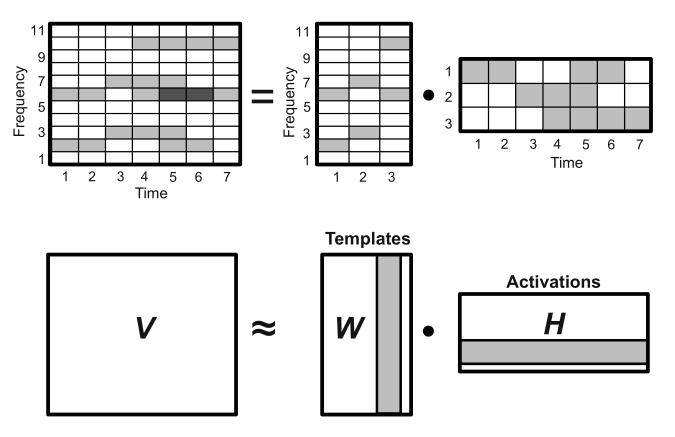
\includegraphics{img/nmf.png}

The problem is formulated as a non-convex optimisation problem

\[(\boldsymbol{W},\boldsymbol{H}) = \mathop{\mathrm{argmin}}_{\boldsymbol{W},\boldsymbol{H}>0} \left\lVert\boldsymbol{V}-\boldsymbol{W}\boldsymbol{H}\right\rVert\]

The implemented cost function \(C=\left\lVert\boldsymbol{V}-\boldsymbol{W}\boldsymbol{H}\right\rVert\) is the euclidean norm \(L_2\).
The matrices \(\boldsymbol{V}\) and \(\boldsymbol{H}\) are decomposed into \(N\) column vectors,
\(\boldsymbol{V}=(v_1,\ldots,v_N)\) and \(\boldsymbol{H}=(h_1,\ldots,h_N)\), which implies
\(\forall i\in\left\{1,\ldots,N\right\},v_i = \boldsymbol{W}h_i\).
By imposing the orthogonality constraint \(\boldsymbol{H}{\boldsymbol{H}}^{\top}=I\),
we obtain the \textbf{K-means} clustering property.
The values of \(\boldsymbol{W}\) and \(\boldsymbol{H}\) can be initialized randomly
and are therefore \emph{learned} iteratively.

Reinforcing a sparsity constraint was proposed in (Cont \protect\hyperlink{ref-cont_2006}{2006})
for spectral factorisation since pitch templates correspond to \emph{discrete}
frequency values.
Moreover, a subset of pitch templates are activated simultanuously
in a musical piece, especially in the case of a piano piece.

Finally, single pitch estimation is performed on rows of \(\boldsymbol{H}\).

Unfortunally, our implementation of this algorithm
did not give successful results, we use
the API provided in for testing (Müller \protect\hyperlink{ref-muller_2015}{2015}).

\begin{Shaded}
\begin{Highlighting}[]
\ImportTok{from}\NormalTok{ muallef.plot.nmf }\ImportTok{import}\NormalTok{ plot\_NMF\_factors}

\ImportTok{import}\NormalTok{ pandas }\ImportTok{as}\NormalTok{ pd}
\ImportTok{import}\NormalTok{ librosa}
\ImportTok{from}\NormalTok{ LibFMP.B }\ImportTok{import}\NormalTok{ plot\_matrix}
\ImportTok{from}\NormalTok{ LibFMP.C8 }\ImportTok{import}\NormalTok{ NMF}

\NormalTok{fs }\OperatorTok{=}\NormalTok{ fur\_elise.sampleRate}
\NormalTok{x }\OperatorTok{=}\NormalTok{ fur\_elise.signal}
\NormalTok{N\_fft }\OperatorTok{=} \DecValTok{2048}
\NormalTok{H\_fft }\OperatorTok{=} \DecValTok{1024}

\NormalTok{X }\OperatorTok{=}\NormalTok{ librosa.stft(x, n\_fft}\OperatorTok{=}\NormalTok{N\_fft, hop\_length}\OperatorTok{=}\NormalTok{H\_fft)}
\NormalTok{V }\OperatorTok{=}\NormalTok{ np.log(}\DecValTok{1} \OperatorTok{+}\NormalTok{ np.}\BuiltInTok{abs}\NormalTok{(X))}
\NormalTok{freq\_max }\OperatorTok{=} \DecValTok{2000}

\CommentTok{\# plot input spectrogram}
\NormalTok{\_ }\OperatorTok{=}\NormalTok{ plot\_matrix(V, Fs}\OperatorTok{=}\NormalTok{fs}\OperatorTok{/}\NormalTok{H\_fft, Fs\_F}\OperatorTok{=}\NormalTok{N\_fft}\OperatorTok{/}\NormalTok{fs, figsize}\OperatorTok{=}\NormalTok{(}\DecValTok{8}\NormalTok{, }\DecValTok{5}\NormalTok{))}
\NormalTok{\_ }\OperatorTok{=}\NormalTok{ plt.ylim([}\DecValTok{0}\NormalTok{, freq\_max])}
\NormalTok{plt.show()}
\end{Highlighting}
\end{Shaded}

\includegraphics{/mnt/my_passport/Backups/2017_11_06_2016_05_16_DELL/D/INSA/GM/GM5/muallef/book_files/figure-latex/nmf-1.pdf}

\begin{Shaded}
\begin{Highlighting}[]
\NormalTok{K }\OperatorTok{=}\NormalTok{ V.shape[}\DecValTok{0}\NormalTok{]}
\NormalTok{N }\OperatorTok{=}\NormalTok{ V.shape[}\DecValTok{1}\NormalTok{]}
\NormalTok{R }\OperatorTok{=} \DecValTok{30}

\CommentTok{\# Initialize and plot random matrices W, H}
\NormalTok{W\_init }\OperatorTok{=}\NormalTok{ np.random.rand(K,R)}
\NormalTok{H\_init }\OperatorTok{=}\NormalTok{ np.random.rand(R,N)}
\NormalTok{plot\_NMF\_factors(W\_init, H\_init, W\_init.dot(H\_init), fs, N\_fft, H\_fft, freq\_max)}

\CommentTok{\# Calculate and plot NMF decomposition}
\end{Highlighting}
\end{Shaded}

\includegraphics{/mnt/my_passport/Backups/2017_11_06_2016_05_16_DELL/D/INSA/GM/GM5/muallef/book_files/figure-latex/nmf-2.pdf}

\begin{Shaded}
\begin{Highlighting}[]
\NormalTok{W, H, V\_approx, V\_approx\_err, H\_W\_error }\OperatorTok{=}\NormalTok{ NMF(V, R, W}\OperatorTok{=}\NormalTok{W\_init, H}\OperatorTok{=}\NormalTok{H\_init, L}\OperatorTok{=}\DecValTok{200}\NormalTok{, norm}\OperatorTok{=}\VariableTok{True}\NormalTok{)}
\NormalTok{plot\_NMF\_factors(W, H, W.dot(H), fs, N\_fft, H\_fft, freq\_max)               }
\end{Highlighting}
\end{Shaded}

\includegraphics{/mnt/my_passport/Backups/2017_11_06_2016_05_16_DELL/D/INSA/GM/GM5/muallef/book_files/figure-latex/nmf-3.pdf}

\begin{Shaded}
\begin{Highlighting}[]
\BuiltInTok{print}\NormalTok{(}\SpecialStringTok{f"V error approximation = }\SpecialCharTok{\{}\NormalTok{V\_approx\_err}\SpecialCharTok{\}}\SpecialStringTok{"}\NormalTok{)}
\end{Highlighting}
\end{Shaded}

\begin{verbatim}
V error approximation = 3.429512976534373
\end{verbatim}

The obtained \(\boldsymbol{V}\) matrix is close to the input spectrogram,
the matrices are all sparse as expected.
Nevertheless, the matrices are fuzzy therefore pitch templates
and their activations are not clear.
The NMF factorisation as is, might not render better results than Klapuri's.
In fact most of pitch templates correspond to multiple note mixtures,
the results can be enhanced by initializing \emph{pitch-informed constraints}
where \(\boldsymbol{W}\) is initialized to MIDI pitch classes.
It can however be very useful method for separating different sound sources.

\pagebreak

\hypertarget{temporal-segmentation}{%
\section{Temporal segmentation}\label{temporal-segmentation}}

\hypertarget{introduction-2}{%
\subsection{Introduction}\label{introduction-2}}

Temporal segmentation is the task of finding time boundaries
of audio objects, in the case of music signals the audio
objects in question are the musical \emph{notes}.

A musical note's \textbf{onset} is defined as the time it starts,
and its ending time is the \textbf{offset}.

\begin{figure}
\centering
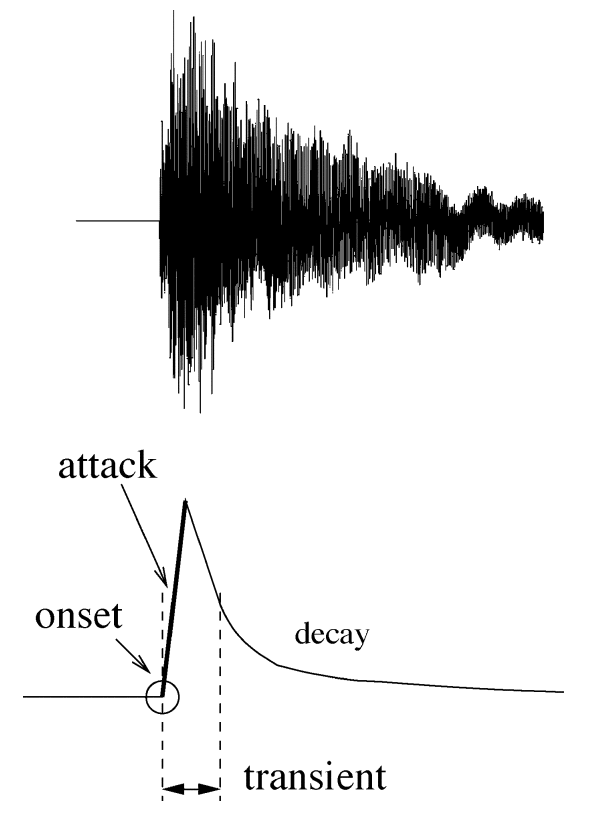
\includegraphics[width=0.5\textwidth,height=\textheight]{img/onset.png}
\caption{IEEE transactions on speech and audio processing, vol.~13, no. 5, september 2005}
\end{figure}

The signal form varies according to instruments.
The onset profile in the image above corresponds to
an instrument producing sudden energy bursts such as
a pinched-chord instrument (piano, guitar, etc),
or a percussive instrument,
unlike bowed-chord instruments and wind instruments
that do no exhibit such energy bursts.
In both cases, the spectral flux, changes in energy,
and/or harmonic distribution are analysed in order
to estimate onset times.

\begin{figure}
\centering
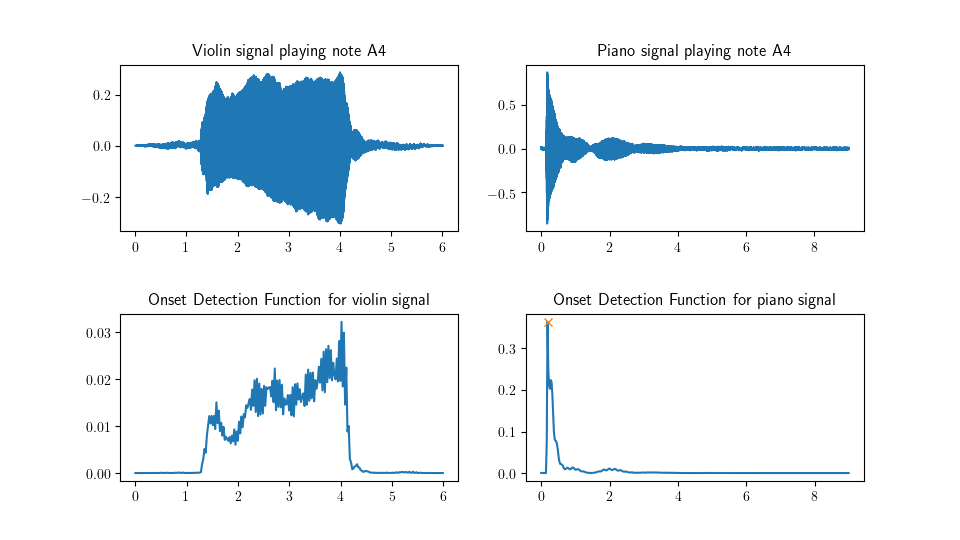
\includegraphics{plot/onset_profiles.png}
\caption{(left) a violin onset profile (right) a piano onset profile}
\end{figure}

The general onset estimation model is a three-step pipeline (Brossier \protect\hyperlink{ref-brossier}{2006})

\begin{enumerate}
\def\labelenumi{\arabic{enumi}.}
\tightlist
\item
  Computing an \textbf{Onset Detection Function (ODF)} that
  characterizes change in energy and/or harmonic content
  in a music signal.
  The change is measured in the time domain, frequency domain,
  phase domain, or complex domain for analysing onsets
  of sounds of different natures.
\item
  Calculate a smooth \textbf{threshold function} as ODFs
  tend to be sensitive to the slightest changes, therefore
  providing a threshold for viable onset candidates.
\item
  \textbf{Peak-picking} local maxima of the ODF that are
  greater than the calculated threshold.
\end{enumerate}

\hypertarget{onset-detection-function-odf}{%
\subsection{Onset Detection Function (ODF)}\label{onset-detection-function-odf}}

We present a few functions that analyse different features
of a musical sound that correspond to subsets of musical sources.

\hypertarget{high-frequency-content-hfc}{%
\subsubsection{High Frequency Content (HFC)}\label{high-frequency-content-hfc}}

The proposed function (Masri and Bateman \protect\hyperlink{ref-hfc}{1996}) favours wide-band energy bursts
over changes in amplitude modulation, and accords a stronger weight
to high frequency spectral bins.

\[D_{\text{HFC}}[n] = \sum\limits_{k=1}^{N}
    k\cdot\left\lVert X[n,k]\right\rVert^2\]

The function emphasises high frequency energy bursts,
which makes it more adapted to percussive onsets than
than bowed-strings or wind instruments. (Brossier \protect\hyperlink{ref-brossier}{2006})

\hypertarget{phase-deviation}{%
\subsubsection{Phase Deviation}\label{phase-deviation}}

A different approach proposed by (Bello and Sandler \protect\hyperlink{ref-bello}{2003}), where the function
evaluates phase difference that can help identify \emph{tonal}
onsets as well as percussive onsets.

\[D_{\Phi}[n] = \sum\limits_{k=0}^{N}
    \left\lvert \hat{\varphi}[n, k] \right\rvert\]

where

\begin{itemize}
\tightlist
\item
  \(\mathrm{princarg}(\theta) = \pi + ((\theta + \pi) mod (-2\pi))\)
\item
  \(\varphi(t, f) = \mathrm{arg}(X(t, f))\)
\item
  \(\hat{\varphi}(t, f) = \mathrm{princarg} \left( \frac{\partial^2 \varphi}{\partial t^2}(t, f) \right)\)
\end{itemize}

The phase deviation function can result in false positives as
phase changes occur in noisy signals.

\hypertarget{complex-distance}{%
\subsubsection{Complex Distance}\label{complex-distance}}

Another ODF is presented in (Duxbury et al. \protect\hyperlink{ref-duxbury}{2003}) that qualifies changes in both
magnitude and phase in order to detect percussing \emph{and} tonal onsets.

\[D_{\mathbb{C}}[n] = \sum\limits_{k=0}^{N}
    \left\lVert\hat{X}[n, k] - X[n, k]\right\rVert^2\]

where
\(\hat{X}[n, k] = \left\lvert X[n, k]\right\rvert \cdot e^{j\hat{\varphi}[n, k]}\)

The presented function combines spectral difference and phase-based approaches,
by borrowing the phase deviation function from (Bello and Sandler \protect\hyperlink{ref-bello}{2003})

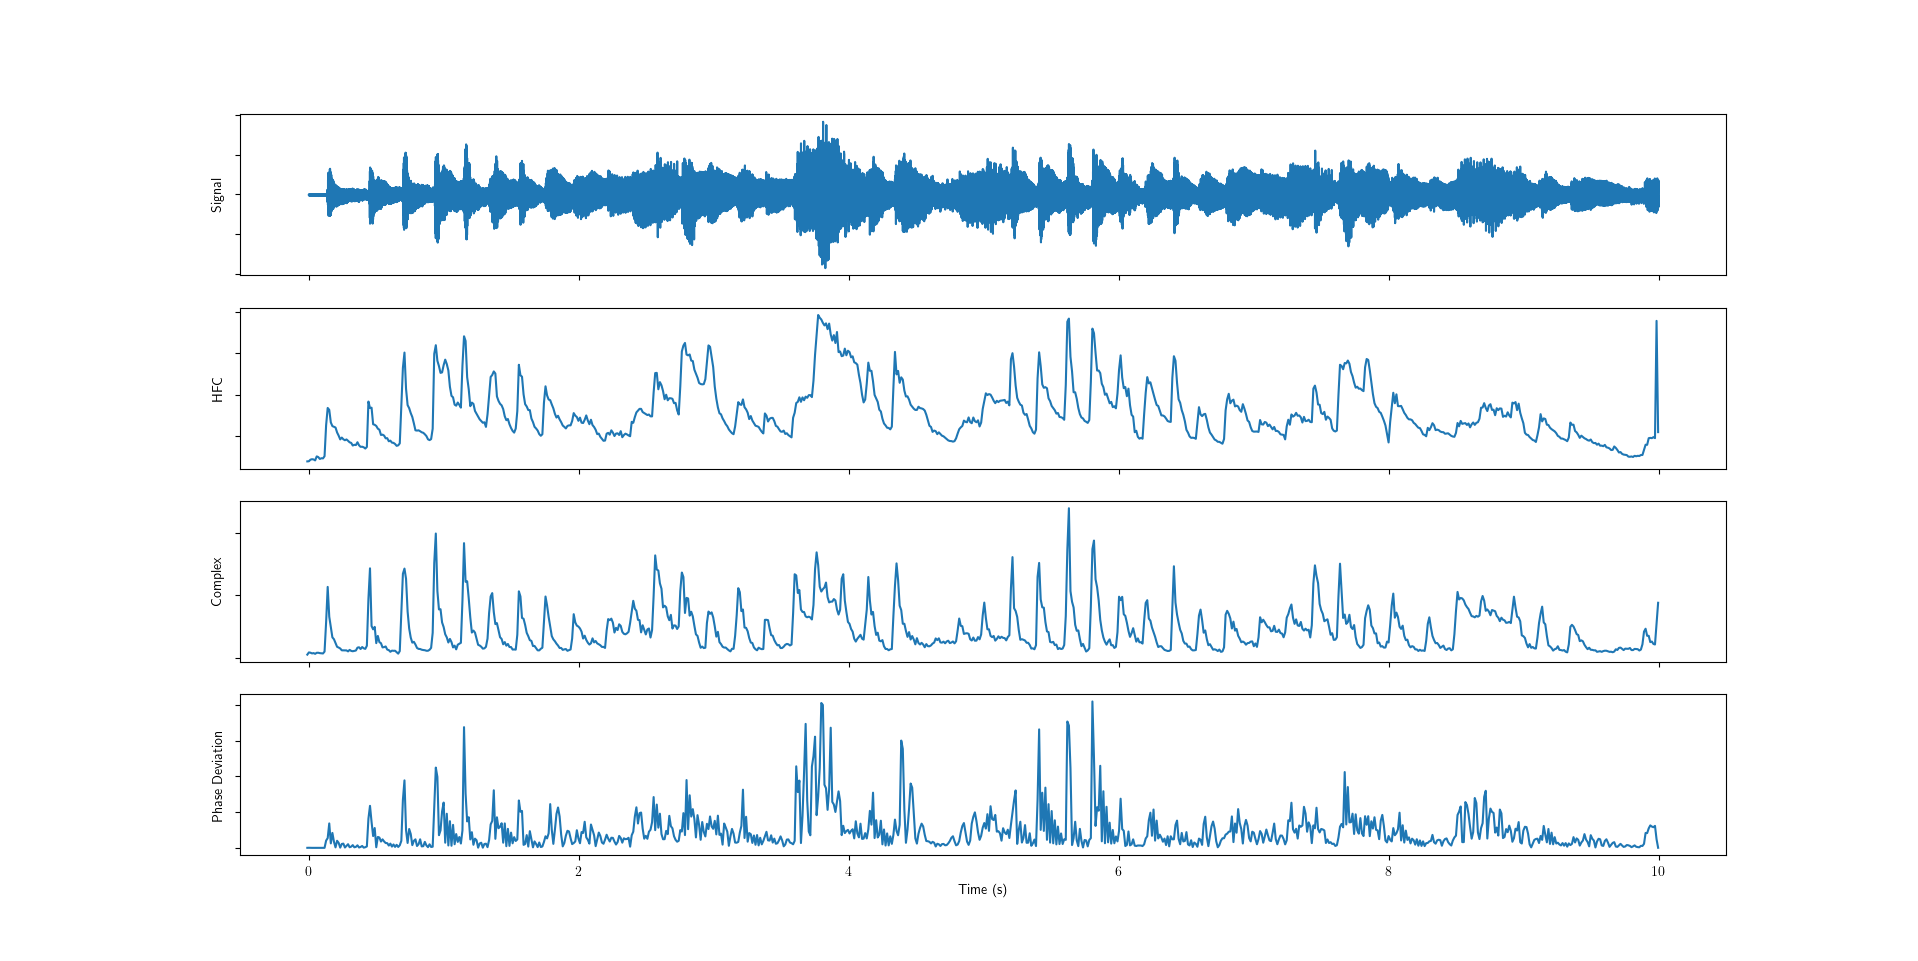
\includegraphics{plot/odf.png}

\hypertarget{thresholding-peak-picking}{%
\subsection{Thresholding \& Peak-picking}\label{thresholding-peak-picking}}

Since Onset Detection Functions are usually sensitive
to the slightest perturbations, false positives belong
to a subset of the local maxima of the ODF.
In order to filter such values, a smoothed version of the ODF
can serve as threshold for eliminating insignificant peaks.

A windowed moving average is a good threshold function,
it is defined as the convolution product of the ODF
with the window function.
In our implementation we have used a Hann window as it
limits the aliasing phenomenon in spectras.

\hypertarget{results}{%
\subsection{Results}\label{results}}

We apply our onset detection pipeline to the same
audio sample of Beethoven's ``Für Elise''.

\begin{Shaded}
\begin{Highlighting}[]
\ImportTok{from}\NormalTok{ muallef.onset }\ImportTok{import}\NormalTok{ Onset}

\NormalTok{fur\_elise.cut(stop}\OperatorTok{=}\DecValTok{5}\NormalTok{)}
\NormalTok{fs }\OperatorTok{=}\NormalTok{ fur\_elise.sampleRate}
\NormalTok{x }\OperatorTok{=}\NormalTok{ fur\_elise.signal}
\NormalTok{t }\OperatorTok{=}\NormalTok{ fur\_elise.time()}

\NormalTok{onset }\OperatorTok{=}\NormalTok{ Onset(x, fs, method}\OperatorTok{=}\StringTok{\textquotesingle{}complex\textquotesingle{}}\NormalTok{)}
\NormalTok{onsets }\OperatorTok{=}\NormalTok{ onset()}

\NormalTok{fig, ax }\OperatorTok{=}\NormalTok{ plt.subplots(}\DecValTok{2}\NormalTok{, }\DecValTok{1}\NormalTok{, sharex}\OperatorTok{=}\VariableTok{True}\NormalTok{)}
\NormalTok{fig.set\_figheight(}\DecValTok{6}\NormalTok{)}
\NormalTok{\_ }\OperatorTok{=}\NormalTok{ fig.suptitle(}\StringTok{"Onset detection of Beethoven\textquotesingle{}s }\CharTok{\textbackslash{}"}\StringTok{Für Elise}\CharTok{\textbackslash{}"}\StringTok{"}\NormalTok{, fontsize}\OperatorTok{=}\DecValTok{16}\NormalTok{)}
\NormalTok{\_ }\OperatorTok{=}\NormalTok{ ax[}\DecValTok{0}\NormalTok{].set\_title(}\StringTok{"Segmented time signal"}\NormalTok{)}
\NormalTok{\_ }\OperatorTok{=}\NormalTok{ ax[}\DecValTok{0}\NormalTok{].plot(t, x)}
\ControlFlowTok{for}\NormalTok{ on }\KeywordTok{in}\NormalTok{ onsets:}
\NormalTok{    \_ }\OperatorTok{=}\NormalTok{ ax[}\DecValTok{0}\NormalTok{].axvline(x}\OperatorTok{=}\NormalTok{on, color}\OperatorTok{=}\StringTok{\textquotesingle{}red\textquotesingle{}}\NormalTok{)}
\NormalTok{\_ }\OperatorTok{=}\NormalTok{ ax[}\DecValTok{1}\NormalTok{].set\_title(}\StringTok{"Complex difference ODF"}\NormalTok{)}
\NormalTok{\_ }\OperatorTok{=}\NormalTok{ ax[}\DecValTok{1}\NormalTok{].plot(onset.onsetTime, onset.onsetFunction)}
\NormalTok{\_ }\OperatorTok{=}\NormalTok{ ax[}\DecValTok{1}\NormalTok{].set\_xlabel(}\StringTok{\textquotesingle{}Time (s)\textquotesingle{}}\NormalTok{)}
\NormalTok{plt.show()}
\end{Highlighting}
\end{Shaded}

\includegraphics{/mnt/my_passport/Backups/2017_11_06_2016_05_16_DELL/D/INSA/GM/GM5/muallef/book_files/figure-latex/onset_complex-1.pdf}

\pagebreak

\hypertarget{conclusion}{%
\section{Conclusion}\label{conclusion}}

Great strides have been made in the field of Music Information
Retrieval pertaining to Automatic Music Transcription,
resulting in satisfactory results for certain underlying
tasks, namely onset detection and single pitch estimation.
Nevertheless, most AMT problems remain open as researchers
worldwide study and apply new concepts everyday.

In the scope of this project, we have explored well-established concepts
of onset detection and single pitch estimation, and succeeded in obtaining
satisfactory results.
We have as well explored two different approaches of multi-pitch estimation
and obtained relatively coherent results with Klapuri's method,
but unfortunally failed in applying Non-Negative Factorisation
as we hoped.

As this is our second attempt in approaching AMT,
we have been able to study closely core concepts of AMT,
and deeply explore the core difficulty of AMT systems
that is \emph{Multi-pitch Estimation}.
As research has lead us to studying several methods and approaches
to this problem, we had to restrict the study to two algorithms
that are robust, mathematically sound and appreciated by the MIR community.

I have held interest for this subject for quite some time,
partly because I am a violinist myself but also because
of my fondness of the employed mathematical principles.
Most importantly, this project requires application of various
mathematical notions as well as computer science skills
hence serving as a demonstration of acquired knowledge
throughout the Masters program.
This open problem is more suited to a PhD thesis subject or
as a full-time focus research, we have attempted to do as much
as we could to accomplish with very little time.

\pagebreak

\hypertarget{references}{%
\section*{References}\label{references}}
\addcontentsline{toc}{section}{References}

\hypertarget{refs}{}
\begin{cslreferences}
\leavevmode\hypertarget{ref-bello}{}%
Bello, J. P., and M. Sandler. 2003. ``Phase-Based Note Onset Detection for Music Signals.'' In \emph{2003 IEEE International Conference on Acoustics, Speech, and Signal Processing, 2003. Proceedings. (ICASSP '03).}, 5:V--441. \url{https://doi.org/10.1109/ICASSP.2003.1200001}.

\leavevmode\hypertarget{ref-benetos_2013}{}%
Benetos, Emmanouil, Simon Dixon, Dimitrios Giannoulis, Holger Kirchhoff, and Anssi Klapuri. 2013. ``Automatic Music Transcription: Challenges and Future Directions.'' \emph{Journal of Intelligent Information Systems} 41 (December). \url{https://doi.org/10.1007/s10844-013-0258-3}.

\leavevmode\hypertarget{ref-brossier}{}%
Brossier, Paul M. 2006. \emph{Automatic Annotation of Musical Audio for Interactive Applications}.

\leavevmode\hypertarget{ref-yin_2002}{}%
Cheveigné, Alain de, and Hideki Kawahara. 2002. ``YIN, a Fundamental Frequency Estimator for Speech and Music.'' \emph{The Journal of the Acoustical Society of America} 111 (4): 1917--30. \url{https://doi.org/10.1121/1.1458024}.

\leavevmode\hypertarget{ref-cont_2006}{}%
Cont, Arshia. 2006. ``Realtime Multiple Pitch Observation Using Sparse Non-Negative Constraints,'' 6.

\leavevmode\hypertarget{ref-duxbury}{}%
Duxbury, Chris, Juan Pablo Bello, Mike Davies, and Mark Sandler. 2003. ``COMPLEX DOMAIN ONSET DETECTION FOR MUSICAL SIGNALS,'' 4.

\leavevmode\hypertarget{ref-feynman}{}%
Feynman, Richard. 1965. ``The Feynman Lectures on Physics Vol. I Ch. 47: Sound. The Wave Equation.'' \url{https://www.feynmanlectures.caltech.edu/I_47.html}.

\leavevmode\hypertarget{ref-klapuri}{}%
Klapuri, Anssi. 2006. ``Multiple Fundamental Frequency Estimation by Summing Harmonic Amplitudes,'' 6.

\leavevmode\hypertarget{ref-lahat_spectral_1987}{}%
Lahat, M., Russell J. Niederjohn, and David A. Krubsack. 1987. ``A Spectral Autocorrelation Method for Measurement of the Fundamental Frequency of Noise-Corrupted Speech.'' \emph{IEEE Trans. Acoustics, Speech, and Signal Processing}. \url{https://doi.org/10.1109/TASSP.1987.1165224}.

\leavevmode\hypertarget{ref-hfc}{}%
Masri, Paul, and Andrew Bateman. 1996. ``Improved Modelling of Attack Transients in Music Analysis-Resynthesis,'' 4.

\leavevmode\hypertarget{ref-muller_2015}{}%
Müller, Meinard. 2015. \emph{Fundamentals of Music Processing - Audio, Analysis, Algorithms, Applications}. Springer. \url{https://www.audiolabs-erlangen.de/fau/professor/mueller/bookFMP}.

\leavevmode\hypertarget{ref-ross_average_1974}{}%
Ross, M., H. Shaffer, A. Cohen, R. Freudberg, and H. Manley. 1974. ``Average Magnitude Difference Function Pitch Extractor.'' \emph{IEEE Transactions on Acoustics, Speech, and Signal Processing} 22 (5): 353--62. \url{https://doi.org/10.1109/TASSP.1974.1162598}.

\leavevmode\hypertarget{ref-schroeder_period_1968}{}%
Schroeder, Manfred R. 1968. ``Period Histogram and Product Spectrum: New Methods for Fundamental-Frequency Measurement.'' \emph{The Journal of the Acoustical Society of America}. \url{https://doi.org/10.1121/1.1910902}.

\leavevmode\hypertarget{ref-NNMF}{}%
Smaragdis, P., and J. C. Brown. 2003. ``Non-Negative Matrix Factorization for Polyphonic Music Transcription.'' In \emph{2003 IEEE Workshop on Applications of Signal Processing to Audio and Acoustics (IEEE Cat. No.03TH8684)}, 177--80. New Paltz, NY, USA: IEEE. \url{https://doi.org/10.1109/ASPAA.2003.1285860}.

\leavevmode\hypertarget{ref-wiki:nyquistshannon}{}%
Wikipedia. 2020. ``Nyquist--Shannon Sampling Theorem.'' \emph{Wikipedia}. \url{https://en.wikipedia.org/w/index.php?title=Nyquist\%E2\%80\%93Shannon_sampling_theorem\&oldid=941933031}.

\leavevmode\hypertarget{ref-yeh_thesis}{}%
Yeh, Chunghsin. 2008. ``Multiple Fundamental Frequency Estimation of Polyphonic Recordings,'' 153.
\end{cslreferences}

\end{document}
